\begin{center}
\footnotesize\noindent\fbox{
	\parbox{\textwidth}{
Definire una procedura iterativa basata sul metodo di Newton per approssimare \(\sqrt\alpha \), per un assegnato \(\alpha > 0\). Costruire una tabella dove si riportano le successive approssimazioni ottenute e i corrispondenti errori assoluti (usare l'approssimazione di Matlab di \(\sqrt\alpha \) per il calcolo dell'errore) nel caso in cui \(\alpha=5\) partendo da \(x_0=5\).
	}
}\end{center}

\noindent Di seguito si riportano la procedura e la tabella richieste, ed il codice usato per costruirla.

\lstinputlisting[language=Matlab]{cap2/es4_function_impl.m}

\begin{center}
	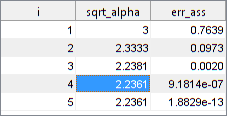
\includegraphics[scale=1]{cap2/2_4.png}
\end{center}

\lstinputlisting[language=Matlab]{cap2/es4_function.m}
